
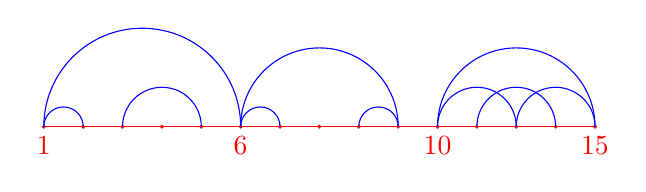
\begin{tikzpicture}[scale=0.5]
\centering
\label{staircasedecompisition}

\foreach \i in {1,...,14} {
        \draw[red] (\i,1) -- (\i + 1,1);
        \filldraw[red] (\i,1) circle (1pt);
 }
\draw[red] (15,1) -- (14,1)node[pos=0.0,below] {15};
\draw[red] (11,1) -- (10,1)node[pos=0.0,below] {10};
\draw[red] (6,1) -- (5,1)node[pos=0.0,below] {6};
\draw[red] (1,1) -- (2,1)node[pos=0.0,below] {1};
\filldraw[red] (15,1) circle (1pt);

\draw[blue, thin] (1,1) arc(180:0:2.5);
\draw[blue, thin] (1,1) arc(180:0:0.5);
\draw[blue, thin] (3,1) arc(180:0:1);
\draw[blue, thin] (6,1) arc(180:0:2);
\draw[blue, thin] (6,1) arc(180:0:0.5);
\draw[blue, thin] (9,1) arc(180:0:0.5);
\draw[blue, thin] (11,1) arc(180:0:2);
\draw[blue, thin] (11,1) arc(180:0:1);
\draw[blue, thin] (13,1) arc(180:0:1);
\draw[blue, thin] (12,1) arc(180:0:1);


\end{tikzpicture}